\chapter{Boat}

\keywords{walking meditation method}

\noindent Walking meditation is a more energetic alternative to the
sitting posture. Find a path, or an area with enough free space to take
a few steps, walking back-and-forth. Even though we are walking, our
attention is directed inward. We are not walking \emph{to} some place,
we are using the walking posture to develop the mind.

An outdoors, private location is ideal, but indoors in a large enough
room is also good.

Determine two points with a clear path between. This could be two trees,
or a couple of pieces of furniture. A short path might be fifteen paces,
a longer one about thirty paces long. Stand at one end, and start
stepping toward the other end mindfully with a clear intention to stay
with your meditation object, such as the breath, or the physical
sensations of the moving body. Keep your gaze lowered, looking at a few
steps in front of you. At the other end of the path, stop and wait for a
couple of breaths. Keeping your intention immersed in the meditation,
turn around, and start walking in the other direction.

Hold your hands in a way that allows you to maintain the continuous
inner attention. Most people prefer clasping the hands in front. It is
not the exact position that matters, but slinging the hands around tends
to be distracting.

\clearpage
\thispagestyle{empty}\mbox{}
\photoFullBleedPlaceholder{%
  TODO: Illustration of walking meditation.%
  \illustration{Walking Meditation Posture}%
  \label{illus-walking-meditation}%
}
\clearpage

Adjust your walking speed to suit your energy level and meditation
object. Some people do walking meditation with fast and determined
steps, other people take slow and careful steps. The suitable speed may
change even during one session. Experience the variations and find what
suits your practice and mental background at that time and place.

\keywords{manipulating feelings, self-importance}

Walking meditation used to stress me out. I believed that it was useful,
but that the technique was too loose and didn't involve precise enough
details about how to do it. I felt I wanted a checklist to go through
and verify if I was doing it right or not.

I kept wanting to walk \emph{to somewhere} so that I would \emph{feel
different}. I would start a walking meditation session between two
trees, but it felt like I was not doing anything, so I kept changing how
I walked to manipulate how I was feeling. `Walk faster, that will be it.
Slow down, and focus. Try breathing like this, and stepping like that,
until it feels different.'

It was also important that other people saw that I was doing something
important. So I would walk back-and-forth until I started to wear a
visible track in the grass on the ground. That was the proof, `I have
done something, I can see it, and \emph{they} can see it!'

Notice how much this kind of struggle is driven by the question, `How
can I feel better about myself?' The motivation is centred on
\emph{manipulating} feelings, not on \emph{understanding} them, how they
arise and cease. Self-importance is not a helpful attitude for practice.
Our desire identifies some external sign and it becomes terribly
important for us to see it, and to let others see it as well. That
\emph{important} track in the grass I made (which probably disappeared
by next dawn) is one example. Articulating it to ourselves when this is
happening already changes our attitude toward the process.

A helpful attitude to practice can be to approach it as if we were doing
something completely ordinary, but to bring along a sense of exploration
and to remember that the benefit is not a wordly goal, there aren't any
stakes to win or to lose. It can also help to \emph{reduce} the
meditation time. It's impressive to do three hours of continuous walking
meditation, but the pressure becomes stressful. How about ten minutes of
meditation? Although it's not major news, it might be fun and
interesting.

\keywords{stopping thinking, mindfulness in the head, internal monologue, control, ordinary practice}

Thinking tends to be strong and self-oriented when we see mindfulness,
consciousness, or meditation as something happening in our head. From
that perspective, mindfulness becomes something `I have to do in my
brain'.\footnote{Cf. Chapter 4, `Mindfulness Mania' in
  \href{https://www.goodreads.com/book/show/44439993-why-i-am-not-a-buddhist}{Why
  I Am Not a Buddhist by Evan Thompson}} This undersells mindfulness as
being merely a rag-doll in the puppet theatre of the brain. Although
that picture suits our favourite idea that we are in control of the
show, it is a narrow view of reality.

\enlargethispage*{\baselineskip}

Cognition is a much more complex and more inclusive system of processes
than that. You can notice how your attention, or whole personal attitude
can change, for example when moving from one building to the next, or
from indoors to outdoors. Your body responds being in a new environment,
the different social context changes your behaviour, a large number of
internal and external factors are involved in creating the perception
you experience as `my mind'. Cognition, or the mind, includes a
networked system of processes operating in unison, taking incoming
signals from a wide area around our bodies. As we experience more of it
as it is happening, it becomes apparent that we don't have the cords to
pull on and make the mind dance to our will.

The thinking and reasoning mind is an instrument which we use for a
motivating purpose. It's not the `good reason' which motivates us, it's
the motivation which makes us find a good reason. Don't try to get to
the end of thinking, notice what is motivating you to think. Letting
that go, the thinking will be let go. The inner rumination can be a form
of comforting oneself, imagining as if we had control in a certain
situation, or trying to regain control over something which already
happened. This is like thinking about the rain: it is going to rain
whether we are thinking about it or not.

If we \emph{can} do something useful about a problem, that's satisfying
to know. If we can't, because it is completely beyond our control, at
least we can know that, and give up chewing ourselves about it.

Thinking tends to have a focused verbal object. When we shift into a
wider, more fluid mode of attention, however, the mind can't put words
to it, and we change into a non-verbal, wordless mode; we perceive the
world around us through this.

The state of non-thinking seems to receive a mystical air, like an
advanced stage of meditation. We don't ask other meditators how much
they use internal self-talk, do we? When you put the question to people,
it turns out that some people don't conduct an internal monologue at
all.\footnote{\href{https://www.psychologytoday.com/us/blog/pristine-inner-experience/201110/not-everyone-conducts-inner-speech}{Not
  Everyone Conducts Inner Speech (psychologytoday.com)}} It's a shocking
surprise to them when they find out that other people talk to themselves
in their head. Others self-talk occasionally, while still others do it
continuously without a break. It is a spectrum, like various positions
on a dial. Personally we are used to doing a particular level of
self-talk, but the level at which we engage this mental faculty is a
habit we can adjust.

If you feel caught in thinking while walking, expand your area of
awareness to include a wider field of cognition. Remember the attitude
of gentle listening, directing attention away from the eyes and the
head.\footnote{Cf. page 117, Gently Listening in
  \href{https://forestsangha.org/teachings/books/alert-to-the-needs-of-the-journey?language=English}{Alert
  to the Needs of the Journey by Ajahn Munindo (forestsangha.org)}} Keep
your eyes lowered on the walking path in front of you. You can visualize
seeing in all directions with your body, or seeing the path with your
feet, through the sensations of touch and pressure. Open your attention
to encompass the entire body as one moving sensation. Open attention
further out to the immediate environment of the walking path.

Short meditations which fulfil their purpose are better than long
periods spent with anxiety about the clock. The purpose is not
generating more stress. The purpose is clarity of mind and being at
ease. Practising, staying with, abiding and dwelling in the space where
stress is relaxed.

\clearpage

\keywords{observing experience, sense-contact}

At the beginning of a meditation session, we collect our attention by
watching the breathing, or the physical sensations of walking
step-by-step. We can't expect alertness and balanced intelligence from
an agitated, excited mind, and so establishing at least some calmness is
essential.

The calm mind is suitable for investigation. What can a happy person
learn from the teaching of the Buddha? What can an unhappy person learn?
Or, what about someone who just feels okay with nothing else special
going on?

We are observing our experience, the signs of impermanence, the
beginning and ending of feelings and thoughts, and how they appear,
change and disappear. Investigating for ourselves gives the words of the
teachings meaning and direct usefulness.

Our experiences manifest through the senses. Forms and colours are
perceived by the eye; sounds by the ear; smells by the nose; tastes by
the tongue; touch, hot and cold by the body; and the mind perceives
thoughts, memories, and other mental processes.

\keywords{three feelings, impermanence}

The experiences appear to us in three qualities, or feelings
(\emph{vedanā}): They may be pleasant, and we feel attracted to them;
they may be unpleasant, and we would rather distance ourselves from
them; or they may be neutral, and their presence doesn't bother us. An
aspect of the neutral feelings is that they, like the breath, can be
experienced as pleasant when we pay attention to them.

\clearpage

The appearance and cessation of the experience are not within our direct
control. The necessary condition for feeling is the contact between a
sense-base, a sense-object, and the attention which is directed there.
With this contact established, the sensation appears on its own. When
the sense-contact breaks, or our attention turns somewhere else, the
sensation disappears.

The happy person who is experiencing pleasant sensations can learn from
investigating them. The attractive impression leads us to cling to the
pleasant sensation, if we forget that this dependent condition is
unreliable. The sensations don't belong to us. It is not possible to
keep, it has no deeper essence, it is empty of self.

The unhappy person who is experiencing unpleasant, painful sensations,
can understand that this condition is not going to last. We can see that
it is superfluous to wind ourselves up with anger or hatred. When action
is required, we act, when waiting with patience is enough, we wait.

The person who feels they are living in a neutral, grey world, can avoid
to give themselves over to carelessness and foggy confusion. This
neutral condition is not going to be permanent either, and if we make
errors through lack of alertness, the result can be painful and
dangerous. It can be like running into a wall or falling into a hole in
the fog.

The impermanence and emptiness fundamentally changes our view, it
reorganizes our values.

The Buddha described feelings as, `all things converge on feeling.' The
eye sees forms, the ear hears sounds, the body feels touch, and so on.
The sense-base makes contact with the sense-object. If attention is
present, there is contact, and the result is the feeling.

Feeling draws our attention to it like a magnet. Remembering the
sequence in the suttas:

\begin{quote}
Rooted in desire, friend, are all things.\\
Born of attention, are all things.\\
Arising from contact, are all things.\\
Converging on feeling are all things.

\bigskip

\quoteRef{%

\href{https://suttacentral.net/an10.58}{AN 10.58}, Rooted

}
\end{quote}

\keywords{feeling as not-self, feelings as bubbles, overcoming anger}

This is the point where we complicate the matter. If we see it as a
transient, unreliable phenomena, we don't make a problem out of it. We
don't form attachments, craving doesn't have a basis to arise and we
don't become stressed. The Buddha compared feeling to the bubbles on the
surface of the water when it is raining heavily.\footnote{\href{https://suttacentral.net/sn22.95}{SN
  22.95}, A Lump of Foam} They appear quickly, and disappear. How could
there be anything in a bubble which we can hold onto?

But our ingrained habit is to assume that this feeling is `me', or
`mine'. From that, craving is born, either a desire to have more of it
or the desire to get rid of it. While we are spending our time reacting
to attraction and repulsion, the underlying compulsive tendencies
(sensual craving, hatred and delusion, i.e. the three \emph{āsavas}) are
fuelled and grow stronger in the mind.

There seems to be a lot of cleaning-up to do in the mind, but it's worth
it. Overcoming anger, for example, is an extremely productive part of
practice. It is an easy mental state to recognize and hence an easy
target to shoot at. Even small progress gives us an inner understanding
about ourselves and the way the Buddhist practice works. The effects of
anger are painful, it makes us sick, we lose our intelligence, and it is
destructive both to our personal and professional relationships. Greed
tends to be sticky, we know we shouldn't but we still want it; in
confusion we are lost; we fear getting close to fear; but it is easy to
want not being enraged. Being free from anger is a relief, and every
step of progress makes the next step easier. Once our head cools down,
what remains is a sense of self-respect and the resolution to practice.

\keywords{fear and anxiety}

If we are in a dangerous or uncertain situation, naturally we begin
thinking about what should we do. Fear and anxiety are going to arise
because there is good reason for it. The emotion of fear carries the
information of possible danger, the emotion of anxiety implies an
uncertain outcome. Fear makes us cautious, and this is useful: I
wouldn't want to ride in a car with a driver who is not afraid of
crashing.

What should we expect from meditation? We might think that \emph{if we
were good meditators} we would be able to stop the fear and anxiety. If
we could just apply the right technique or remember the right words,
these annoying mind states would disappear. Notice in this motivation
the desire which strives for control. We are wishing for our situation
to be different from the way it is, to manipulate and end it.

Our attitudes influence the direction the feeling develops. Certainly,
we can make it worse. All the while, we are internally debating with
ourselves, imagining the situation to play out one way or another. The
internal dialogue of anxiety is a form of trying to control the events
around us. We try re-interpreting what we see in a way that fits our
earlier view of the situation. Once such a feeling has already appeared,
though we can't change or fix it, we are still part of the process.
Awareness of the mind state keeps it within safe bounds, but gives it
space to let it run its course and end.

When I am waiting for my luggage at the airport, I feel anxious -- did
they lose my luggage? I have done all I needed to do, and there is
nothing more I can do now. I feel anxiety because the situation is, in
reality, uncertain. As a practice, I recollect that I have enough space
to stay with this feeling. There is no need to hurry things up, the
anxiety can stay as long as it needs to be there.

We can't stop it, but we can stop making it worse. If there is a danger,
we do what is necessary. If there is no danger at the moment, but we
feel anxiety, we can understand that \emph{the anxiety is not the
danger}, and we can mindfully stay present without fear of the feeling.

\keywords{contemplating the body, simplify the method, slowing down thinking, BUD-DHO}

How does the feeling appear, when observed through the body? Where do we
feel it? When did it start? Is it changing? As a feeling in the body, is
it that bad? This type of investigation will not give us control, but it
develops an understanding that the feeling is not the danger, and we
don't have to continue the internal fight for control.

If the thoughts are not slowing down, we can occupy the thinking mind
with a thought which we determine, instead of allowing it to run in
every direction. A mantra, such as `BUD-DHO' can be used in this case.
It is a simple method to collect our scattered attention and make it fit
to work for our benefit.

If meditation feels too complicated, simplify it down to the essence.
Lots of complicated steps only increase the sense of unfamiliarity and
doubt.

\enlargethispage*{\baselineskip}

One breath, one BUD-DHO. On the in-breath, we internally recite the
first half of the mantra, BUD-. The breath pauses in the middle for a
moment. On the out-breath we recite the other half, -DHO. BUD-DHO.

The essence is the understanding which stops you, and leaves peace where
`you' had been. The peace originates from the senses withdrawing, and
the flow of attention turning inwards. The seeking stops, because what
is here is enough, and there is no need to go anywhere.

\keywords{sadness at emptiness}

The first impression of emptiness can be focused on loss, and we feel
sadness. With experience we learn to recognize more refined aspects of
emptiness, in which we don't own, but haven't lost anything: this
emptiness is liberating.

When the wordly goals turn out to be empty and not as important as we
thought, there can be a feeling of sadness, disorientation, we're not
sure which way to continue.

This is like being unsure about ourselves when waking up, a new world
taking the place of the dream. After the disorientation passes, a quiet
joy arises in the mind. The ongoing wakefulness recognizes the happiness
in the present. Our values reorganize themselves. We don't look for
external strength and security, because dependent conditions are
uncertain, unsatisfactory, and their pursuit without end is tedious.

Who is suffering? This experience, how is it changing? Where is the
peace now? Where is the understanding now? Experience is not a problem
to solve. Awareness stays with the experience and comprehends it.

\enlargethispage*{2\baselineskip}

Turn attention to the moment before you ask the question: Who is asking
whom? This the trick of the narrating mind. It imagines there is
somebody to talk to, somebody to criticize or complain to. But the voice
speaking into the microphone, the questioner and the respondent are one
and the same, and between question and answer there is neither: only the
listening.

\keywords{stories of the world, BUD-DHO}

BUD-DHO, breathing in, breathing out: the stories of the world are not
interesting for us. When the questioning attention stops the words in
the mind, this is enough. Listening silence fills the pause, and the
answer is the present experience.

Meditation based on the breath and BUD-DHO is easy to adapt to informal
situations. In everyday situations, whether by using a mantra, or
wordlessly, simplify the practice until you can clearly recognize the
right attitude. The simple practice of watching the breath doesn't add
any more complications to the comings and goings of the world. We don't
have to solve experience, it is enough to watch and listen.

\keywords{tudong story, self-criticism, self-support, aversion subverting Dhamma}

One time I was on a walk, out in the countryside, wandering from town to
town with a backpack. I was sleeping in a small tent, and going
alms-round each day at the nearest village in the hope of receiving some
food for the day. We call this practice \emph{tudong}. I printed maps on
A4 sheets of paper, on which I would usually write notes as well. I had
been walking for a few days at that point, tracking on the paper which
paths I followed; noting where I found good camping spots; marking where
I received alms-food in the villages; and so on. It is a kind of travel
log or journal. When I get back to the monastery, I scan the maps and
type up the notes.

This was a rainy and windy day, and I was walking in the middle of
nowhere on a muddy road. I sat down to rest, and I thought, `Let's mark
up this last section of the route on the map.' I took a look in the
plastic folder where I kept the maps, and I could see today's map, but
yesterday's map was not there. \emph{I've lost yesterday's map.} With
all the notes.

I must have dropped it sometime earlier when pulling out today's map for
a look. It could be kilometres behind me, in the mud somewhere, or the
wind may have blown it into some corner. I kept thinking, `I've lost
yesterday's map. I can't believe I've lost my map.' I felt so shaken, it
was comically absurd. I hadn't realized how much I treasured these
little notes, it felt like I'd lost a part of my life. I couldn't
remember the last time I was so disappointed.

The Sun was going to set soon, and I still had a lot of distance to
walk. The next morning I had to reach the next town, otherwise I
wouldn't be able to go alms-round, which would mean I wouldn't be eating
that day. (The monk's rules don't allow us to store food from one day to
the next.)

So I couldn't easily turn around and start tracing my way back. I was
sitting there, thinking, `I should let go. It's just some notes. This is
just a state of mind, a good monk would let go.'

But all that didn't sit right. I thought, `What am I afraid of? Why is
it wrong to like that piece of paper? Why is it OK to criticise myself
and push toward the next goal, but not OK to be even a bit
self-supportive? I love doing what I do, and I'm going back for my map!'

I found it about 500 meters behind me. It was floating in a puddle,
soaked, but intact. I lifted it from the water as carefully as if it
were an archaeological artefact. I rolled it up in a towel and it
eventually dried.

Meeting such obstacles is a fruitful practice. That day I learned more
than I volunteered for. It was almost dark by the time I found a place
to camp but everything was well. The next day I did get to the town in
time for alms-round, and a man and two ladies offered me food for the
day.

The values we grow up with in Western culture make it readily acceptable
to think critical, judgmental thoughts about ourselves. When we say, `he
is his own worst critic', this sounds hard, but it is something we
praise. Certain Buddhist terminology fits right in with this, `Give up
your desires! You shouldn't have preferences! Everything is not self!
Let it go!' This mode of attention operates from self-aversion, it
subverts the Dhamma in order to beat ourselves up with it. And although
it's painful to practice this way, we still think that such aversion is
`good'. Fortunately, it doesn't take any special skills to correct
course in the right direction, it's enough to stop going the wrong way.

\keywords{getting things done, four roads to success, iddhipāda}

Doubt and criticism stop everything. The energy to move toward a goal
depends on the faith that that goal makes sense, and the resolution to
put effort into it. We don't have to know how it will work out to the
end, but if we consider the situation, we are ready ask, `What is the
smallest possible step I can do right now?'

The Buddha described the mental tools for success in four categories
called the Paths for Success (\emph{iddhipāda}): enthusiasm, energetic
effort, focused attention and investigation (Figure
\ref{fig-success}).\footnote{Cf.
  \href{https://buddhadhamma.github.io/path-factors-of-concentration.html\#development-of-concentration-in-line-with-the-paths-to-success}{Chapter
  18.6.B. in Buddhadhamma (buddhadhamma.github.io)}, Development of
  Concentration in Line with the Paths to Success} One might call these
tools the `Buddhist Getting Things Done' method.

\keywords{changing plans, meeting obstacles, the best time to learn}

\enlargethispage*{\baselineskip}

You might have heard the saying, `Plans are worthless, but planning is
indispensable'.\footnote{U.S. President Dwight D. Eisenhower used this
  phrase, which he credited to an unnamed soldier.} The plan changes
when we meet the actual circumstances. But when we are improvising the
new route, we utilize the information we gathered while planning.

Investigating the circumstances, considering the worst possible outcome
that is reasonable to expect, if we can at least avoid that, that's
enough to resolve to start. Keep the momentum going, keep the sails in
the wind.

In theory, to learn and practice sounds attractive, but what kind of
situations can we expect to learn from? Looking back, I remember periods
when everything was going well in life and things were under control. At
such pleasant times, I could use and refine the old steps which had
always worked before. When I was feeling terrible, sorry for myself and
complaining, I didn't learn much from that. And when I followed a
routine of trivial, comfortable but grey habits day after day, that
wasn't particularly insightful either.

\clearpage
\null\vfill

\begin{figure}[h]
\caption{The Four Paths to Success (\emph{iddhipāda})}\label{fig-success}

\centering

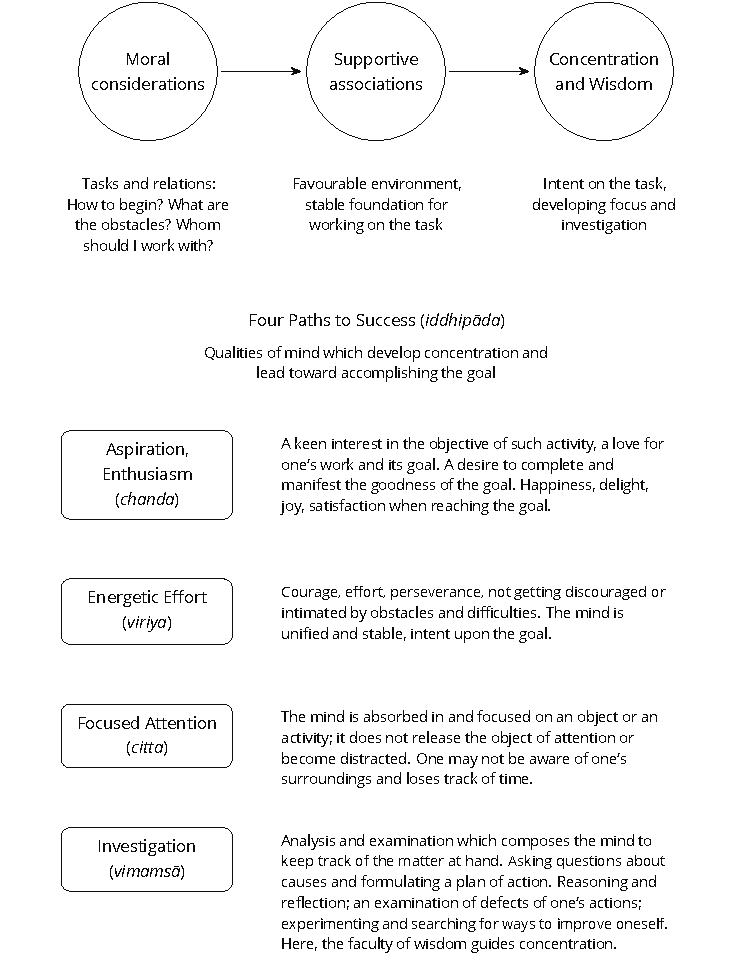
\includegraphics[width=\linewidth]{./manuscript/tex/diagrams/paths-to-success.pdf}

\end{figure}

\vfill\null
\clearpage

Quiet and peaceful times are a blessing. I always appreciate a stable
routine which allows for long periods of concentrated work or dedicated
practice. That said, obstacles and conflicts are guaranteed to arise.

We don't have to worry that meditation is going to solve our every
problem and that we will have nothing left to do. Meditation is not
problem-solving. It is a practice of awareness which overcomes inner
obstacles and faces external problems as they arise. If we have
something important to do, it helps to clear our head first. But merely
sitting on a cushion as if we have transcended all problems, we are
practising ignorance the present, not the awareness of it.

Voluntarily facing obstacles and addressing them skilfully is a golden
chance to develop the mind beyond our preconceived limits. The confused
chaos is rich in the potential to develop and learn in a practical way.

We are not seeking the feeling themselves, not trying to create special
feelings by meditating, or seeking the ideal situation where everything
will pleasantly work for us. Pleasant, unpleasant, neutral feelings will
not, in themselves, give us right understanding if we follow their
influence and react mechanically. Awareness has to notice their
impermanence and uncertainty. With this, we can see what is wholesome
and what is unwholesome in the present situation.

\enlargethispage*{\baselineskip}

\keywords{boat moving on the river, me and mine}

Is meditation practice easy or difficult? A useful image to think about
is how a boat moves on a river. When the boat is packed and burdened
with product-filled crates, it moves heavily and slowly. It is just
barely holding itself above the water.

We want our boat to go fast, don't we? But at the same time, we are
holding onto everything we packed it with. We have to lighten our boat,
and let go of the heavy burden of the self. We create the burden of `me'
and `mine'. We create the impression of `I have been like this. I am
like this. I should be like this.' `That was mine. This is mine. This, I
want to keep. That, I have to get'. This is the weight that is holding
our boat down.

The sense of having enough creates the mental space for generosity.
Contentment is an ongoing part of practice. It is not a fixed state
attached to conditions. Wise action and learning flow like a stream from
contentment: When I think, `I will be ready to do it when I have
\ldots{}', discontent occupies my thoughts and keeps interrupting my
focus on the current situation.

\keywords{wholesome thoughts, peace}

But when I think, `I am not good at it, but I have enough to start',
accepting my current limits gives me energy for action. Then I often end
up doing more than what I thought.

Thinking has a bad reputation in meditation texts, but clear thoughts
create a condition for developing right attitude. Proliferative,
compulsive thinking is a painful experience, but wanting to stop all
thinking also misses the target.

Notice how wholesome thoughts are followed by contentment and peace.
Consciously recollecting one's moral actions establishes a sense of
stability and self-respect. We can trust ourselves to let go of the
superfluous because we feel we already have enough.

If we try to solve it in our head, the practice is going to get
complicated fast. In meditation, awareness through the body is a
reliable guide: Watching the feelings and mind states as they come and
go, we shift our view from being preoccupied with ourselves. We can
leave behind complicated questions because we no longer need the
answers.

\keywords{light boat, enjoyable learning}

What enables us to keep learning and developing? The journey is most
enjoyable when the horizon keeps expanding beyond our previous limits.
We expand the horizon not by travelling far, but by seeing with new
eyes. The desire to hold onto what we think we are creates our current
limits.

The boat is light, when it is empty of me and mine. It can cover great
distances without making drama and fuss. What happens, if we are sitting
in a boat, and somebody runs into us with their boat? We shout at them,
push them away with the oars, and complain about it for the rest of the
day. All this might be justified, but we ruined our day with our own bad
company. It's hard to see the wisdom in that. What happens if an empty
boat floats into our boat? Where did the earlier anger and negative
emotion come from?

We tend to manufacture stories about me and mine, whether based on real
or imagined events. If we take them seriously, and give them reality,
the stories start to control us, and we create problems which didn't
exist before.

\enlargethispage*{\baselineskip}

Sometimes we sit on a meditation cushion and start playing out inner
arguments with puppets of the imagination. It's a serious business! We
have to win! Methodically thinking through a problem is a powerful tool,
but sympathy and kindness toward ourselves is necessary for a
constructive inner dialogue. Otherwise, when the self is talking with
itself, it finds itself in bad company.

\keywords{he who can laugh at himself}

It's surprising how we can wind ourselves up about a situation which
hasn't even happened yet. It helps to keep a pinch of humour in our
side-pocket in case of emergency seriousness. Recollecting a saying of
the Greek philosopher Epictetus, `He who can laugh at himself never runs
out of things to laugh at.'

\keywords{simplicity of the senses, letting go}

In the practice of meditation, we restore right view by returning to the
simplicity of the senses. If stories arise, we observe them from the
perspective of changing conditions. By investigating the senses, we take
a more fundamental level as our basis for attention. Pleasant feeling is
like this, as we are experiencing it. Unpleasant feeling is like this.
Neutral feeling is like this. They have a beginning and an end, they are
changing and empty.

In the practice, the value comes not in accumulating results in a hurry,
but in leaving space for letting go and patience. There are times for
action, but simple patience solves a surprising variety of difficulties.
The sense of being hurt, the feelings of urgency and importance come
from ourselves. Restraint gives us a safe perspective, guarding
ourselves and others. Let us allow our boat to move on in silence.
